\section{Kamerakalibrierung}
%Um einen Punkt, welcher von der Kamera bzw. der Queue-Erkennung erfasst wurde, korrekt in das Spielfeld zu projezieren, müssen folgende Schritte durchlaufen werden:\\
%Der gegebene Punkt, welcher in einem 2D Vektor vorliegt, muss in das gegebene Spielfeldkorrdinatensystem transformiert werden. Hierfür muss das Spielfeld zunächst von der Kamera erkannt werden um anschließend im Kamerakoordinatensystem festgehalten zu werden. Da das Kamerabild eine natürliche Verzerrung des Bildes beinhaltet, muss ebenso diese Verzerrung entzerrt werden. Dies wird mit Hilfe eines bekannten Musters, welches in diesem Projekt ein Schachbrettmuster ist, bewerkstelligt, in welchem signifikante Eckpunkte erkannt, daraus die Verzerrung ermittelt und entzerrt werden. Nachdem dies erfolgt ist, kann ein erkannter und entzerrter Punkt aus der Kamera in das Spielfeldkoordinatensystem übertragen werden. Hierfür muss eine Umrechnung erfolgen, da das Kamerakoordinatensystem oben links den (0,0)-Punkt hat und das Spielfeld unten rechts.

%\subsection{Einleitung}
%Sobald die Anwendung gestartet wird, wird die Kamera verbunden und ein Timer fragt alle 16ms ab, ob die Kalibrierung gestartet werden soll. Wenn dem so ist, wird auf dem Spielfeldbereich ein Schachbrettmuster gerendert und nach jedem Ablauf des Timers, hier dem entsprechend alle 16ms, Fotos aufgenommen. Sobald eine festgelegte Grenze von aufgenommenen Fotos erreicht wurde, werden diese ausgewertet, ob das Schachbrettmuster auf diesen Fotos erkannt wurde. Falls dem nicht so ist, werden erneut Fotos aufgenommen. Ansonsten werden die Eckpunktkoordinaten des erkannten Musters gespeichert und damit die Entzerrung ausgeführt. Im Anschluss kann ein, von der Queue-Erkennung erfasster Punkt, entzerrt und ins Spielfeld übertragen werden.

\subsection{Darstellung des Erkennungsmusters}
Um die Kamera kalibrieren und das Kamerabild bzw. die -punkte entzerren zu können, muss die Kamera ein bekanntes Erkennungsmuster finden und in diesem bestimmte Eckpunkte erfassen und auswerten können. In unserem Projekt wird ein Schachbrettmuster genutzt, von welchem die inneren Eckpunkte erkannt werden. Hierfür muss die Anzahl der Kacheln in der Horizontalen = $Hor$, sowie in der Vertikalen = $Vert$, bekannt bzw. festgelegt sein, um für jede Kachel die selbe Höhe und Breite zu haben und trotzdem die gesamte Höhe und Breite des Spielfeldes abzudecken. Die Höhe und Breite wird wie folgt berechnet:\\
$Hoehe_{Kachel} = \frac{Hoehe_{Game}}{Vert}$, $Breite_{Kachel} = \frac{Breite_{Game}}{Hor}$\\
Nun wird für jedes $i \in [1,Hor]$ alle $j \in [1,Vert]$ eine Kachel gerendert mit den Koordinaten oben links ($i \cdot Hoehe_{Kachel}$, $j \cdot Breite_{Kachel}$) und den Koordinaten unten rechts ($(i+1) \cdot Hoehe_{Kachel}$, $(j+1) \cdot Breite_{Kachel}$). Zudem wird bei jeder neuen Kachel in der Horizontalen die invertierte Farbe der vorherigen Kachel als Grundfarbe gewählt und in der Vertikalen für die erste Kachel die invertiere Farbe der darüber liegenden Kachel gewählt, damit das klassische Schwarz-Weiß-Muster eines Schachbretts visualisiert wird.
\begin{figure}[h]
	\centering
	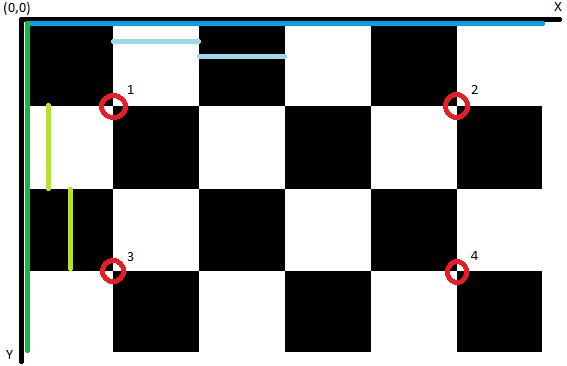
\includegraphics[scale=0.7]{bilder/schachbrett.png}
	\caption{Schachbrettmuster rendern}
\end{figure}

\subsection{Entzerrung des Kamerabildes/Punktes}
Für die Kalibrierung des Kamerabildes mittels eines Patternmusters, muss zwischen zwei Ansichten unterschieden werden. Zum einen sind das die Weltkoordinaten, welche in einem 3D-Koordinatensystem liegen, zum anderen die Bildkoordinaten, welche in einem 2D-Koordinatensystem liegen. In unserem Fall wird in den Weltkoordinaten ein bekanntes Muster bzw. die Erkennungspunkte des Schachbretts festgehalten, um im Anschluss das erkannte Muster auf dem Foto mit diesem abzugleichen und somit die Entzerrungsparameter herauszufinden. Da dies eine festgelegte Anzahl an Erkennungspunkten aufweist, werden genau diese Erkennungspunkte, mit einer festen Kantenlänge für jede Kachel, im Weltkoordinatensystem modelliert. Da die übergebenen Punkte nachher in ein 2D-Koordinatensystem, das vom Spiel, dargestellt werden sollen, werden die Erkennungspunkte des Schachbrettmusters als 2D-Punkte gespeichert:\\
$WeltCoords = (x \cdot a, y \cdot a, 0), a$ = Kantenlänge, $x \in [0,Vert-1], y \in [0,Hort-1]$\\
Nun werden die aufgenommenen Bilder der Kamera von dem, im vorherigen Abschnitt gerenderten, Schachbrettmuster analysiert, ob auf diesen das bekannte Pattern erkennbar ist. Dies wird mit der OpenCV-Methode $findChessboardCorners$ gemacht, welche neben dem aufgenommenem Bild auch die Anzahl der vertikalen und horizontalen inneren Musterpunkte als Parameter übergeben bekommt und, falls alle gefunden wurden, einen Wert ungleich 0 zurück gibt und diese in einem Bildkoordinatensystem festgehalten, ansonsten 0. Falls die Rückgabe ergibt, dass das Muster erkannt wurde, existiert nun für jedes Bild, auf dem das Patternmuster erkannt wurde, ein Bild- und ein Weltkoordinatensystem.
Im Anschluss wird die eigentliche Kamerakalibrierung gestartet, welche durch folgende Formel repräsentiert wird:\\
\[s
\begin{bmatrix}
u\\v\\1
\end{bmatrix}=
\begin{bmatrix}
f_{x} & 0 & c_{x}\\
0 & f_{y} & c_{y}\\
0 & 0 & 1
\end{bmatrix}
\begin{bmatrix}
r_{11} & r_{12} & r_{13} & t_{1} \\
r_{21} & r_{22} & r_{23} & t_{2} \\
r_{31} & r_{32} & r_{33} & t_{3}
\end{bmatrix}
\begin{bmatrix}
X\\Y\\Z\\1
\end{bmatrix}
\]
Als Eingabe werden die Bildkoordinaten als 2D Matrix, sowie die Weltkoordinaten als 3D Matrix der gefundenen Pattern und der Anzahl vertikaler und horizontaler Fixpunkte im Schachbrett übergeben. Aus diesen Parametern wird eine 3x3 Kamera- bzw. intrinsische Matrix, welche den Standpunkt der Kamera in der Welt darstellt, sowie ein Vektor mit den Verzerrungskoeffizienten und die Rotations- und Translationsvektoren, welche die extrinsischen Parameter darstellen. Kurz gefasst werden die Weltkoordinaten zu Kamerakoordinaten unter Verwendung der extrinsischen Parameter und die Kamerakoordinaten zu Bildkoordinaten unter Verwendung der intrinsischen Parameter.
\begin{figure}[h]
	\centering
	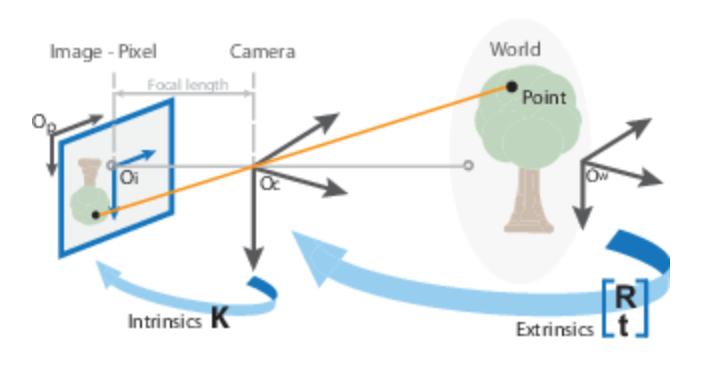
\includegraphics[scale=1.3]{bilder/extrinIntrin.png}
	\caption{Extrinsisch und Intrinsisch}
\end{figure}
Nun sind alle nötigen Eingaben gegeben um einen beliebigen Punkt aus dem verzerrten Bild zu entzerren. Hierfür wird zunächst, mit Hilfe von $undistortPoints$, der Eingabe des 2D Punkts, der Kameramatrix und den Verzerrungskoeffizienten, der eingegebene Punkt entzerrt. Anschließend muss dieser entzerrte Punkt noch korrekt rotiert werden. Hierfür wird eine 2x3 Rotationsmatrix benötigt. Da bisher nur Rotationsvektoren ermittelt wurden, wird zunächst mit $Rodrigues$ der (erste) Rotationsvektor in eine 3x3 Rotationsmatrix konvertiert. Daraufhin werden die ersten beiden Reihen dieser Matrix mit $vconcat$ zu einer 2x3 Matrix umgeformt. Als letzten Schritt wird auf den entzerrten Punkt diese Rotationsmatrix mit $warpAffine$ angewendet um den endgültig entzerrten und rotierten Punkt zu erhalten. Somit besteht nun das vollständige Verfahren einen beliebigen Punkt aus den Bildkoordinaten korrekt in die Weltkoordinaten zu transformieren.

\subsection{Punktübertragung von Kamera ins Spiel}
Der letzte Abschnitt der Kamerakalibrierung stellt das Übertragen eines von der Queue-Erkennung gegebenen Punktes, welcher sich im Kamerakoordinatensystem befindet, in das Spielfeldkoordinatensystem um diesen dann in den Spielmechanismus als Queueposition einzubinden.
Um dies einwandfrei zu ermöglichen, müssen die äußersten Eckpunkte des, von der Kamera erfassten, Schachbrettmusters im Kamerakoordinatensystem bekannt sein. Da allerdings nur die Eckpunkte auf der Innenseite des äußersten Ringes des Schachbretts erkannt werden, müssen die ganz äußersten Eckpunkte wie folgt berechnet werden:\\
$Lila_{min} = Gruen_{min} - Rot_{min}$, 
$Lila_{max} = Rot_{max} - Gruen_{max}$
\begin{figure}[h]
	\centering
	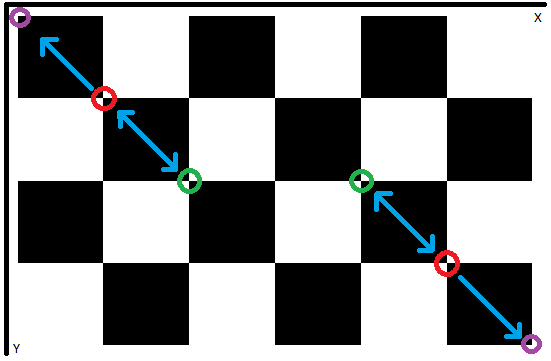
\includegraphics[scale=0.7]{bilder/schachbrettdiff.png}
	\caption{Schachbrettmuster Eckpunkte}
\end{figure}\\
Nun sind die äußersten Eckpunkte des Spielfeldes im Kamerakoordinatensystem bekannt und es ist möglich einen beliebigen 2D Punkt in das Spiel zu projizieren. Hier wird unter zwei Fällen unterschieden. Der übergebene Punkt der Kamera liegt im Spielbereich gdw. $X \in [x_{min}, x_{max}]$ und $Y \in [y_{min},y_{max}]$ gilt.
Sofern dies erfüllt ist, wird der gegebene Punkt mit folgenden Gleichungen jeweils mit der X- und Y-Koordinate umgerechnet :\\
$X = \dfrac{(P.x - MIN.x) \cdot UR}{(MAX.x - MIN.x)}$, 
$Y = \dfrac{(MAX.y - P.y) \cdot OL}{(MAX.y - MIN.y)}$
\begin{figure}[h]
	\centering
	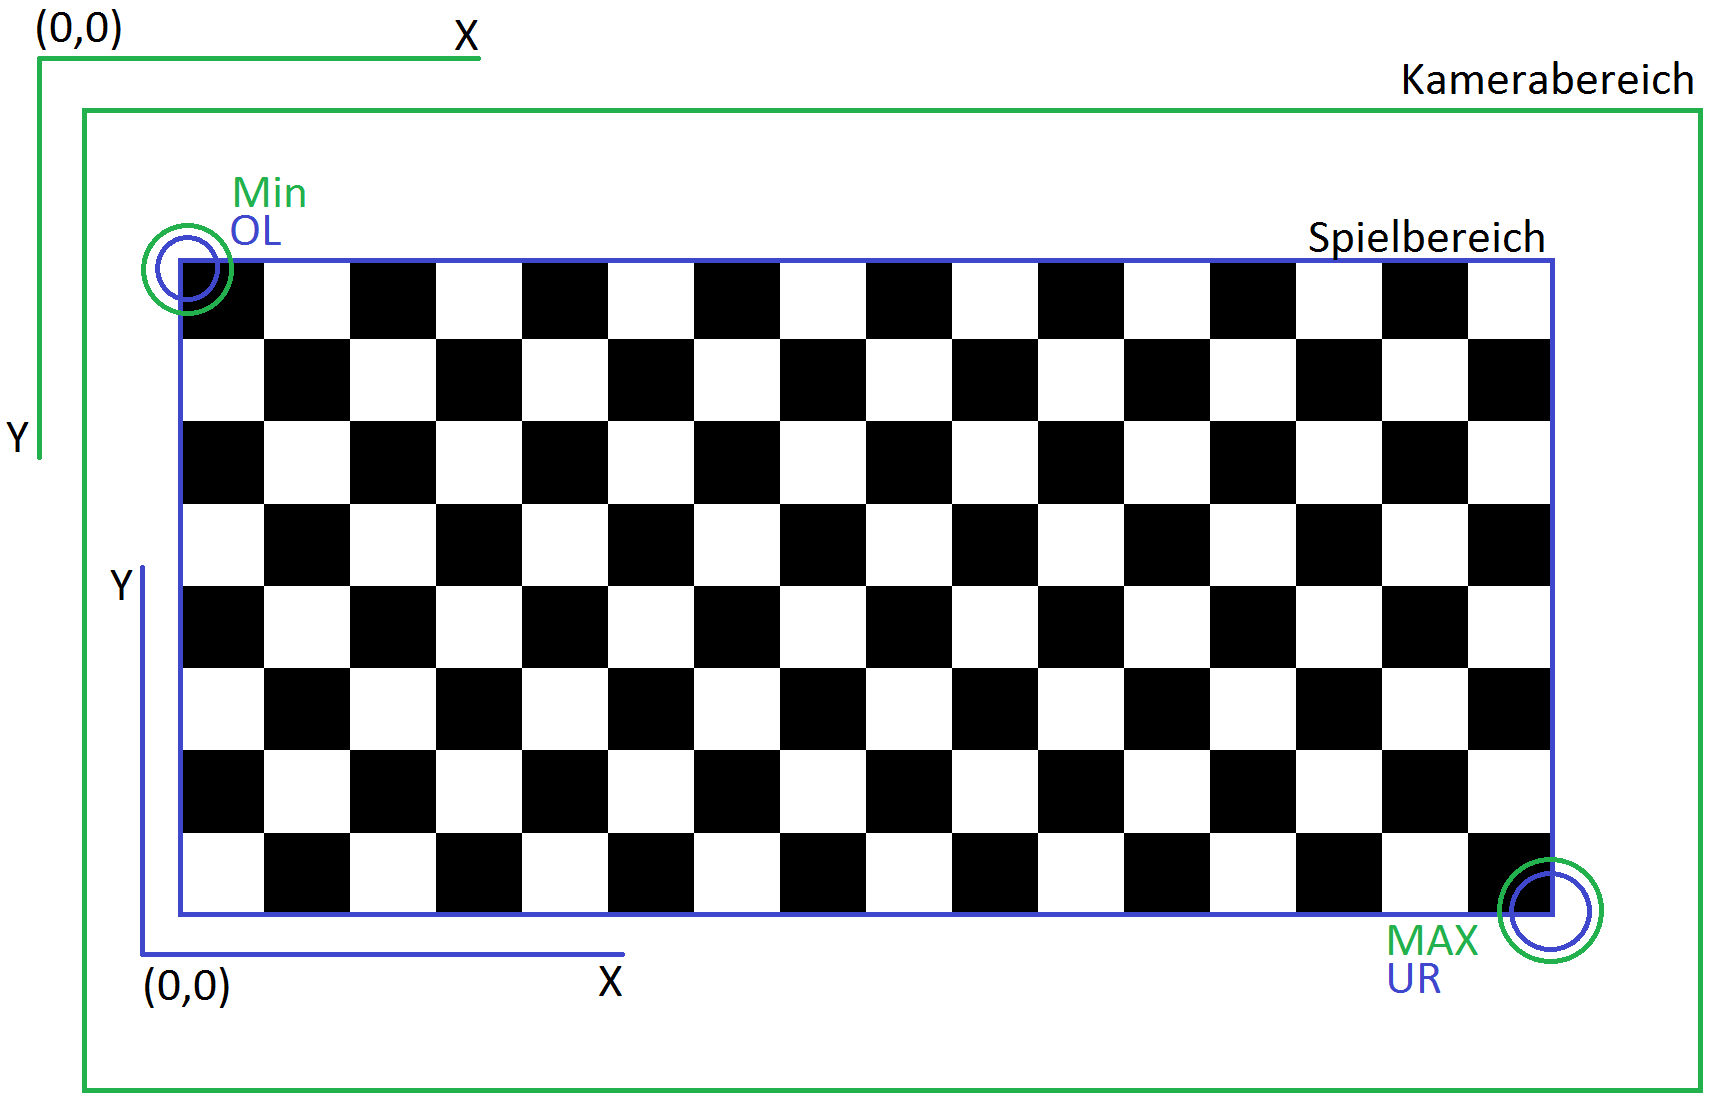
\includegraphics[scale=0.2]{bilder/schachbrettkamera.png}
	\caption{Kamera- und Spielkoordinatensystem}
\end{figure}

\subsection{Zusammenfassung}
Zusammenfassend wurde ein, von der Kamera erfasster, Punkt in das zweidimensionale Spielfeld projiziert. Dafür wurde zunächst ein Muster generiert und angezeigt, in welchem die Kamera bekannte Fixpunkte erkennen und mit diesen das aufgenommene Bild entzerren kann. Mit den Fixpunkten wurden die äußersten Kanten des Musters berechnet und mit diesen der Anfangs gegebene Punkt ins Spiel übertragen.